\documentclass[border=10pt]{standalone}
\usepackage[T1]{fontenc}
\usepackage[default]{sourcesanspro}
\usepackage{tikz}
\usepackage{fontawesome}
\usepackage{xcolor}
\definecolor{Indigo}{RGB}{75,0,130}
\definecolor{ForestGreen}{RGB}{34,139,34}
\usetikzlibrary{arrows.meta,positioning}

\begin{document}
\begin{tikzpicture}[>=Stealth, node distance=2cm and 4cm]
		% Draw the entities
		\tikzset{c/.append style={fill=Indigo!30,rounded corners, align=center, text width=5cm}}
		\tikzset{person/.append style={text width=2.5cm,fill=ForestGreen!30,rounded corners,align=center}}
		\node[person](Alice) {\faFemale{} Alice\\\texttt{10.0.0.1}};
		\node[person, right=of Alice] (Bob) {\faMale{} Bob\\\texttt{10.0.0.2}};

        % Draw the arrows and labels
		\draw[->, thick, Indigo, dashed] (Alice.south) -- node[c] { Ich m\"ochte mit dir sprechen, Bob. \\\texttt{SYN}, \texttt{SEQ} = $x$} ([yshift=-2.5cm]Bob.south);

		\draw[->, thick, Indigo, dashed] ([yshift=-2.5cm]Bob.south) -- node[c] { Ok, lass uns reden Alice!.\\\texttt{SYN, SEQ} = $y$ \texttt{ACK}=$x+1$} ([yshift=-4cm]Alice.south);
		\draw[->, thick, Indigo, dashed] ([yshift=-4cm]Alice.south) -- node[c] { Ok, danke Bob.\\\texttt{ACK}=$y+1$} ([yshift=-6cm]Bob.south);

		\node[below of=Alice, yshift=-5cm] (AliceZeit) {Zeit};
		\node[below of=Bob, yshift=-5cm] (BobZeit) {Zeit};

		% Time line
		\draw[->, thick] (Alice.south) -- node[xshift=-.2cm, rotate=270] {Zeitachse von Alice} (AliceZeit);
		\draw[->, thick] (Bob.south) -- node[xshift=.2cm, rotate=270] {Zeitachse von Bob} (BobZeit);
	\end{tikzpicture}
\end{document}
